\section{Git}
\label{sec:git}

Today, hardly any software project is started without any form of version control system (\texttt{VCS}). It supports developers as a back-up system and living archive of their work, as data generally is ephemeral and can be lost easily \cite[1]{loeliger2012version}. Although there are many different variations offered, some of the most popular today are \emph{Git, Apache Subversion, Mercurial} and \emph{Bazaar}.

\subsection{History}
\label{sec:git-history}
\texttt{Git} was initially published by \emph{Linus Torvalds} on April 7\textsuperscript{th}, 2005 \cite[6]{loeliger2012version}. This was necessary, as the ``free'' version of the then used VCS for the \emph{Linux} kernel development, \texttt{BitKeeper}, was restricted in a way it was not suitable any longer for the community behind it. Furthermore, the search of an already available alternative to the \texttt{BitKeeper} system failed due to an unsatisfying combination of needed features, so \emph{Torvalds} came up with his own VCS flavor, containing all desired functionalities for further \emph{Linux} development (among others) \cite[4]{loeliger2012version}:

\begin{itemize}
  \item Distributed development
  \item Handle thousands of developers
  \item Efficient performance
  \item Support branched development
  \item Free, as in freedom
\end{itemize}

While it was merely a tool for kernel hackers in the beginning, its simplicity quickly made developers use it for other projects too. However, the CLI still scared off people with less programming background, until \texttt{GitHub} came and introduced its Desktop client\footnote{\url{https://desktop.github.com/} -- GitHub Desktop client.}. Today, it is one of many GUIs, which are available for different operating systems\footnote{\url{https://git-scm.com/downloads/guis} -- Git GUI clients on the \texttt{Git} website.} and completely omits the necessity of terminal emulator knowledge when working with \texttt{Git}.

%% Write something, why it is so famous. distributed development - other use cases .. blargh.

\subsection{Technology}
\label{sec:git-technology}
Having decided to use \texttt{Git} as VCS, everything begins with setting up a new respository. This can be made remotely on a service like \texttt{GitHub}, or locally using \texttt{git init}. When initialized a local repository, it can still be published remotely through setting the correct URL using \texttt{git remote} later on \cite[198]{loeliger2012version}.

\subsubsection{Commits}
The next step would be working with the repository. For the most part, this should not influence the developer's workflow in any way, as the \texttt{.git} directory should be automatically hidden in most modern editors to not distract him/herself from the actual work. If the developer succeeded in a sub-task or simply wanted to save the current project state, he/she would create a \emph{commit}.

A \emph{commit} is a snapshot of the current repository's state. While it does not contain a copy of every file and directory in the project tree, it rather compares the current condition with its predecessing snapshot and creates a list of affected files and their changes. Blobs\footnote{\emph{BLOB} -- Binary Large OBject, a file which does not consist of queryable source code.} are either reused, if they remain unchanged or created new, if they were altered\cite[65]{loeliger2012version}.

Every \emph{commit} is organized in a way, that it is chained to its predecessor (\emph{parent}), thus representing a singly linked list with the ability of gaplessly going back from the current state (\emph{head}) to the initial \emph{commit} \cite[204]{dhillon2016}\cite[65]{loeliger2012version}. This is necessary, as it may happen to fix a bug or improve a design decision only by reworking a certain snapshot in the past \cite[151]{loeliger2012version}.

\subsubsection{Branches}

%% Graphic of git branches
\begin{figure} % h-ere, t-op, b-ottom, p-age
    \centering
    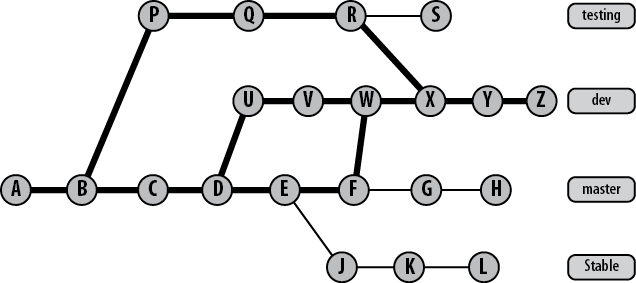
\includegraphics[width=0.8\textwidth]{git-branches.png}
    \caption{A graphic showing the basic structure of branches in \texttt{Git}.\\
    The \textbf{testing} branch was created out of project state ``B'', whereas \textbf{dev} was branched away from state ``D'' and currently holds the \emph{head commit} at ``Z''. In the meantime, \textbf{testing} was merged into \textbf{dev} at state ``R''. In the end, \textbf{dev} contains the commit history of all states connected with the bold line \cite[p. 92f]{loeliger2012version}.}
    \label{fig:git-branches}
\end{figure}
%

Since its early days, \texttt{Git} was used not only as back-up or archive system, but also as code management system. This is possible due to built-in functions, such as the so-called \emph{branched development}, where a current state of the actual development is duplicated and worked on separately. It allows for development to continue in multiple directions simultaneously \cite[89]{loeliger2012version} (see Fig. \ref{fig:git-branches}).

When being part of a remote team, a developer may also \emph{push} his/her own local branches for providing it to others, as well as keeping them for local development and \emph{merging} them back to the main branch after succeeding in his current task \cite[207]{dhillon2016}. Through the use of these possibilities, a responsible administrator keeping track of the development structure is not necessarily required to be appointed in any repository settings. Furthermore, the team may decide members in charge for merges in an agile way, based on the current need.

\subsubsection{Usage in static site development}
The advantages of using \texttt{Git} in static site development are mainly its possibilities of providing a full-featured archive of the content and source code of each project. Seamlessly going back and forth in the website development history makes it easy to navigate between every single content edit, without loosing track of previous and future revisions. In this case, it may work significantly better than using a common database system for content storage.

Furthermore, it is also possible to make use of \texttt{Git} \emph{hooks}. Once a new \emph{commit} is created, a \emph{hook} might take care of invoking the \textbf{build pipeline} as a ``post-receive'' \emph{hook} -- thus, the new website version gets built automatically without requiring any additional user interaction. However, \emph{hooks} should be only used with caution, as they are not distributed the same way as the files tracked in a given repository and also may harm the integrity of their \texttt{Git} repository \cite[p. 285f]{loeliger2012version}.

\section{GitHub}
\label{sec:git-github}

Already mentioned it a few times before (see p. \pageref{sec:jekyll}, \pageref{sec:buildpipelines-markdown} or \pageref{sec:git}), \emph{GitHub} is currently probably the most popular online collaboration platform, hosting not only the source code for the Linux kernel\footnote{\url{https://github.com/torvalds/linux} -- Linux kernel repository on GitHub.}, but also for other huge projects like Google's \emph{TensorFlow}\footnote{\url{https://github.com/tensorflow/tensorflow} -- Tensorflow repository on GitHub.}, Microsoft's \emph{.NET}\footnote{\url{https://github.com/Microsoft/dotnet} -- .NET repository on GitHub.} or Facebook's \emph{React}\footnote{\url{https://github.com/facebook/react} -- React repository on GitHub.}.

\subsection{History}
Tom Preston-Werner, a Ruby programmer from San Francisco and creator of earlier mentioned Jekyll (see ch. \ref{sec:jekyll} on p. \pageref{sec:jekyll}) and \emph{Chris Wanstrath} started developing GitHub in October 2007. After releasing a private beta in January, they released the site to the public on April 10\textsuperscript{th}, 2008 \cite{PrestonWerner2008githublaunch}.

Since then, GitHub grew very fast and quickly gained on popularity throughout the developer landscape, hosting more than 56 million projects today\footnote{\url{https://github.com/about} -- GitHub's ``about'' page.}. Thanks to their generous freemium pricing model, collaborating in open source projects still is for free: A free tier account may hold unlimited open source repositories, working together with unlimited contributors\footnote{\url{https://github.com/pricing} -- GitHub's pricing page.}. All in all it seems, that GitHub turned coding into a truly social activity \cite[416]{loeliger2012version}.

\subsection{Technology}
The main use case for creating a repository on GitHub is the fact, that unlike other privately hosted remote repositories, it offers a wide range of additional services. Services like \emph{Issue tracking, Pull requests} and \emph{Code reviews} leverage the maintainability of source code in a repository, making it easy for each developer to discuss and manage the current project state without the need of switching to a third party application.

%% Screenshot of GitHub in-page editor
\begin{figure} % h-ere, t-op, b-ottom, p-age
    \centering
    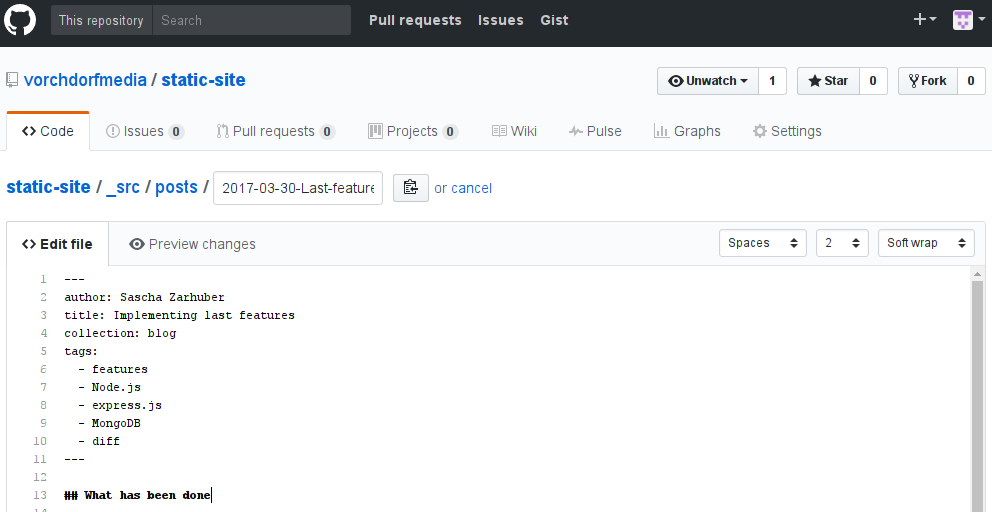
\includegraphics[width=0.9\textwidth]{github-page-editor.png}
    \caption{A Screenshot showing the \emph{In-Page Code Editor} of GitHub. An existing file is selected and ready to be edited. When finished, the user may commit the changes into the repository, so that other contributors also benefit from his/her adjustments.}
    \label{fig:github-page-editor}
\end{figure}
%

Especially for content authors without programming knowledge, the \emph{In-Page Code Editor} might be a very supportive tool, as it provides a clean and easy-to-use frontend for directly adding content to the repository (see Fig. \ref{fig:github-page-editor}). Additionally, the just edited file may not only be committed into the currently selected branch, but also in a newly created branch. Therefore, the source branch stays clean, whereas the edited file may get reviewed by an assigned supervisor, before being ready to get merged.\\
Furthermore, also developers might make use of this feature, especially when a small hotfix is to be made, where it would be too time-consuming to \emph{pull, commit} and \emph{push} from/to the repository \cite[405]{loeliger2012version}.

Pushing to a \emph{gh-pages} branch, or creating a \emph{<username>.github.io} repository, enables the use of GitHub's built-in website hosting service. From there, either a Jekyll project is freshly built, or already compiled static HTML are automatically published to the web -- additionally, custom domains may be used when adding a \texttt{CNAME} file \cite[p. 171f]{dhillon2016}.

\subsection{REST API}
Another significant advantage is the access of GitHub's REST API. Currently existing in its third major release, it almost offers every feature also available graphically in its web interface, as an equivalent JavaScript Object Notation (\emph{JSON}) upon programmatical request. Some services even feature more advanced data through the API than through the UI \cite[410]{loeliger2012version}.

When having the need of including data from a GitHub account into a third party service, a single authenticated HTTP request does the trick. Due to many available endpoints, a developer may quickly find the type information he/she needs to further process data directly from a repository. As an example, a complete listing of a repository's file tree is also possible, without needing to download and unpack an archive file. For one thing, this saves quite some time, for another thing, the requested data is already processed and presented, so that not only file paths are unveiled, but also their direct links and data types.

Furthermore, the API not only offers access to informational data about a given repository, instead, its manipulation through creating commits or uploading a file may also happen. To sum this up, very well documented examples are available on the API page on GitHub, where developers catch a good glimpse, of what is possible overall\footnote{\url{https://developer.github.com/v3/} -- API v3 documentation on GitHub.} \cite[401]{loeliger2012version}.

